% the goal of the project is for each group to improve the system (either mechanical design, add sensor and improve control, or a modeling approach of dynamics of the hand).
% write a proposal of what you want.
% we can add a spring for the fingers to modulate the stiffness of the fingers.

\documentclass[10pt]{article}
	
\usepackage[margin=1in]{geometry}		% For setting margins
\usepackage{amsmath}				% For Math
\usepackage{fancyhdr}				% For fancy header/footer
\usepackage{graphicx}				% For including figure/image
\usepackage{float}
\usepackage{hyperref}
\usepackage{tabto}
\usepackage{cancel}					% To use the slash to cancel out stuff in work
% avoid all eq numbering via:
\usepackage{mathtools}
\mathtoolsset{showonlyrefs}

\usepackage{cite}
\usepackage{url}
\usepackage{amssymb}                % To include mathbb symbols
\usepackage{graphicx}               % In preamble
\newcommand{\mcG}{\mathcal{G}}
\newcommand{\mcU}{\mathcal{U}}
\newcommand{\mcV}{\mathcal{V}}
\hypersetup{colorlinks=true,
            urlcolor=blue}
            
% Set up fancy header/footer
\pagestyle{fancy}
\fancyhead[LO,L]{Wearable Robotics 0360108}
\fancyhead[CO,C]{Final Project - Proposal}
\fancyhead[RO,R]{\today}
\fancyfoot[LO,L]{}
\fancyfoot[CO,C]{\thepage}
\fancyfoot[RO,R]{}
\renewcommand{\headrulewidth}{0.1pt}
\renewcommand{\footrulewidth}{0.1pt}
% \renewcommand{\thesubsection}{(\roman{subsection})}
\renewcommand{\thesubsubsection}{(\roman{subsubsection})}
\usepackage{algorithm}
\usepackage{algorithmic}


%%%%%%%%%%%%%%%%%%%%%%

\begin{document}
\begin{table}[h]
    \centering
    \begin{tabular}{l l l}
        \hline
        Name & ID & Email \\
        \hline
        Elad Siman Tov & - & elad.sim@campus.technion.ac.il \\
        \hline
        Eitan Gerber & - & eitangerber@campus.technion.ac.il \\
        \hline
    \end{tabular}
    \label{tab:personal_info}
\end{table}

% -------------------------------------- %
\section*{Proposal}
We propose to achieve five different grasps using 2 or 3 EMG sensors by training a classifier to determine the desired predefined grasps. The predefined grasps are provided in figure \ref{fig:grasps}. We chose grasps that would be feasible to implement on our hand, given that it is underactuated as it only has 1 motor per finger. We aim to implement our high level control such that when switching between grasps the controller would pass through a neutral position for the hand as illustrated in figure \ref{fig:classifier}.

\begin{figure}[H]
    \centering
    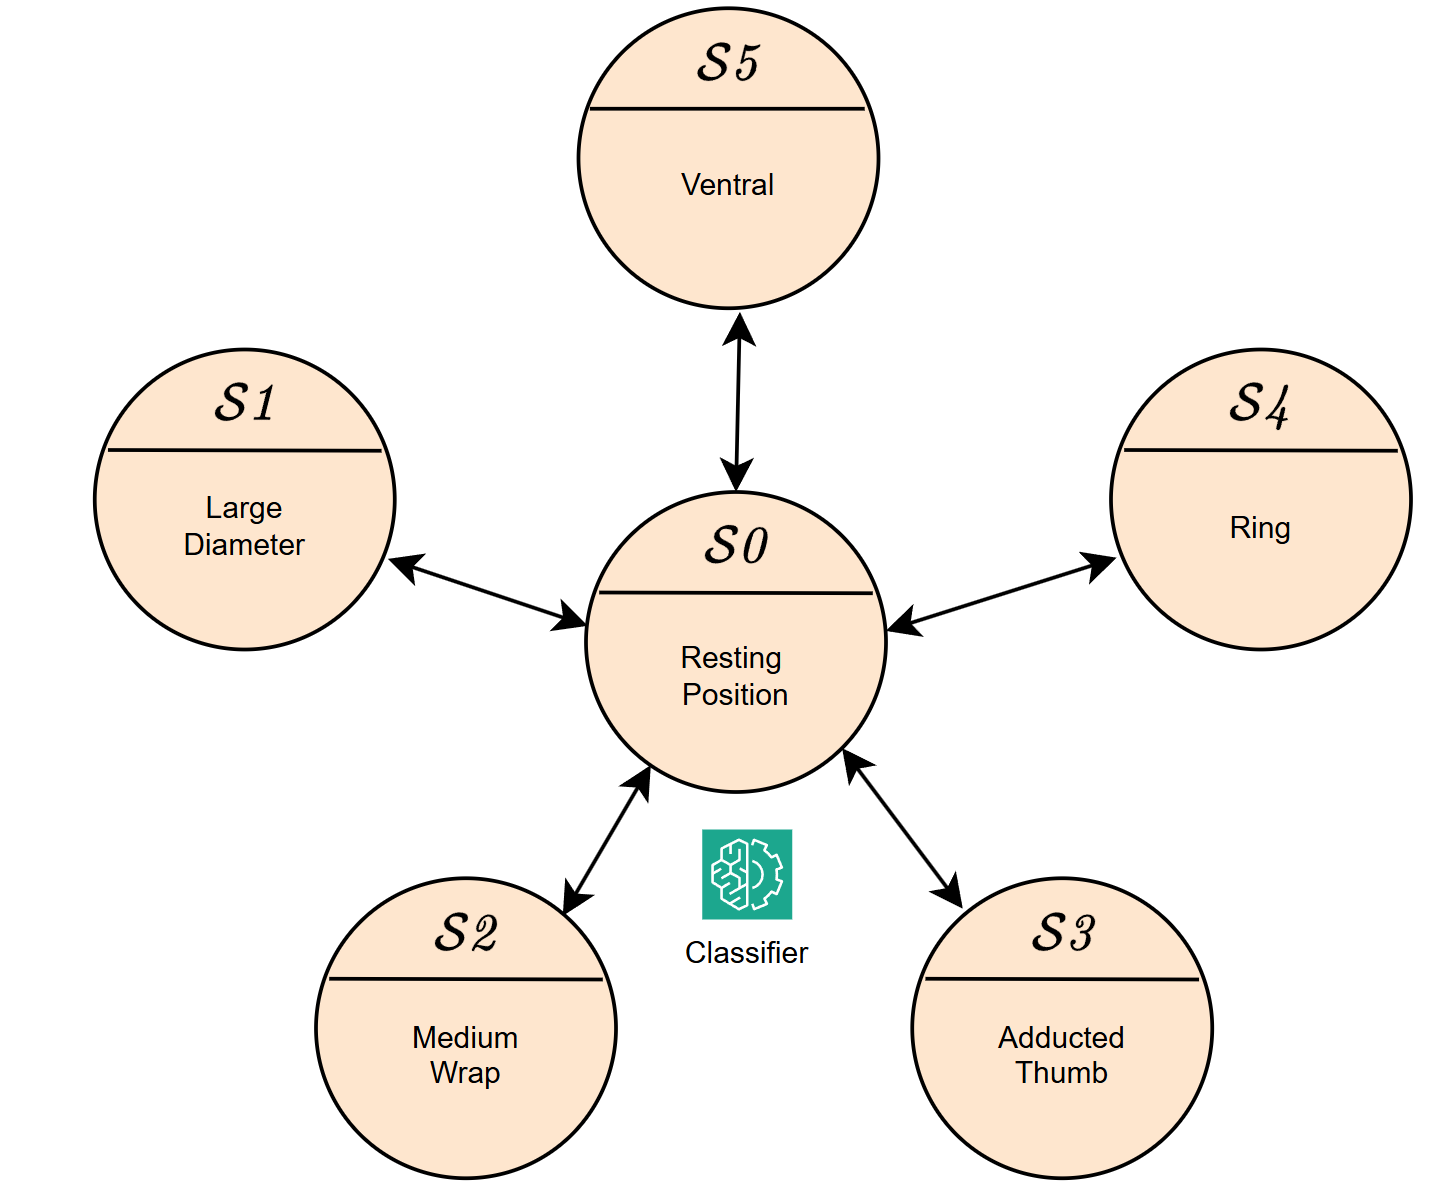
\includegraphics[width=0.7\linewidth]{Final Project/classifier.png}
    \caption{The classifier determines the grasp and switches via the neutral position.}
    \label{fig:classifier}
\end{figure}


\begin{figure}[H]
    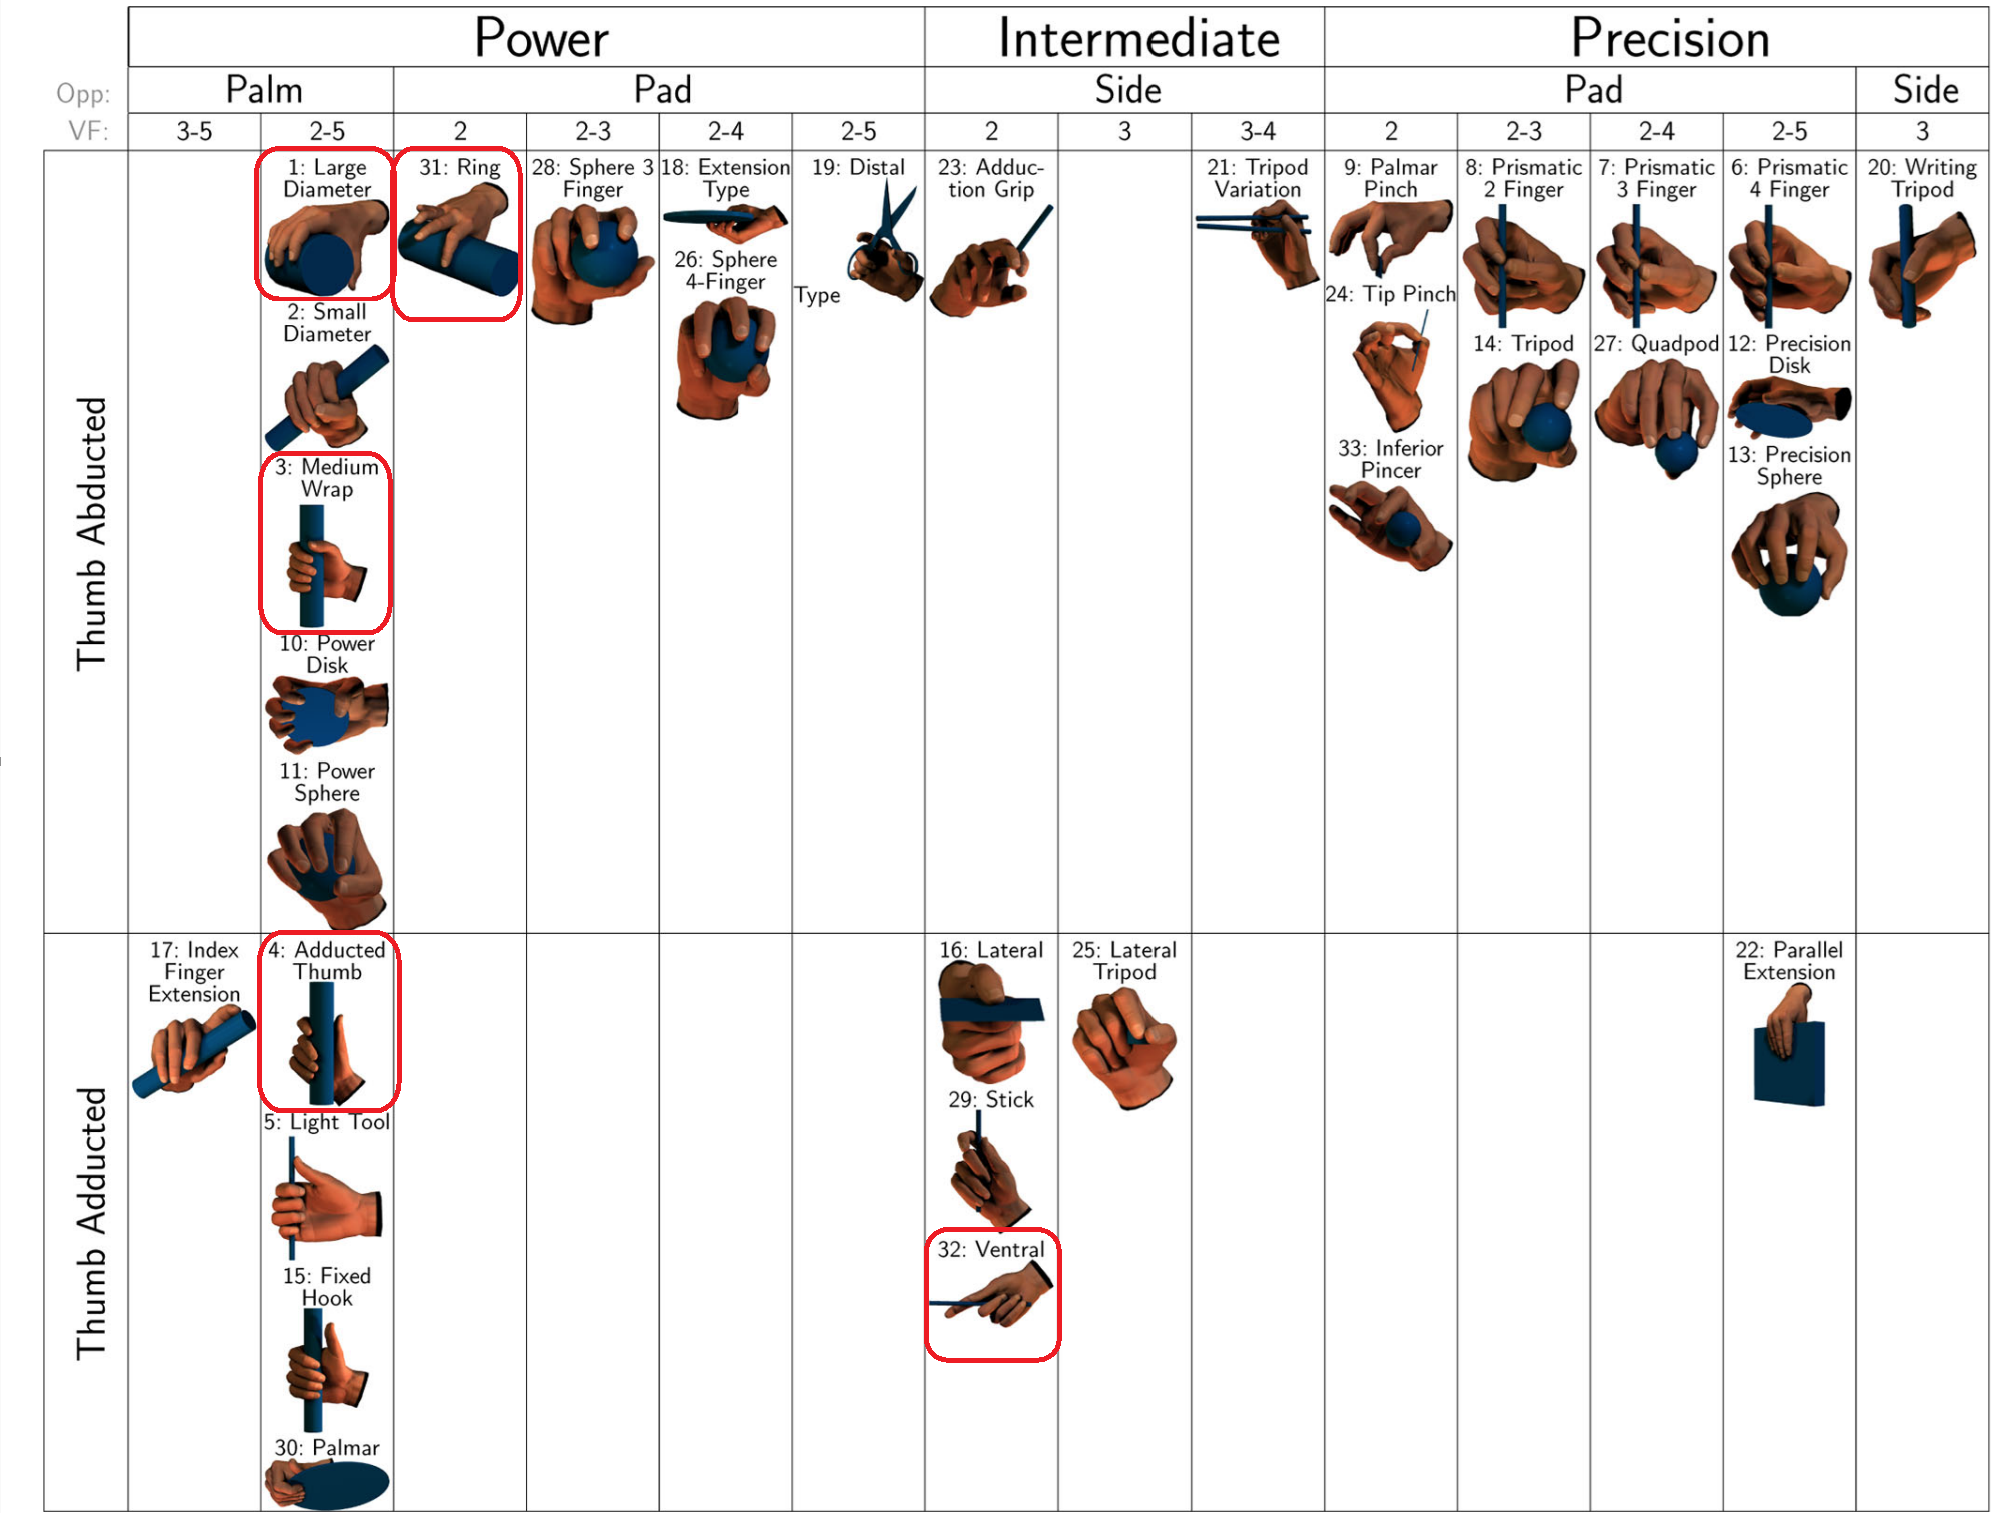
\includegraphics[width=1\linewidth]{Final Project/grasps.png}
    \caption{The predetermined grasps that would be classified and implemented in our robotic hand. Adapted from \cite{7243327}}
    \label{fig:grasps}
\end{figure}
\bibliographystyle{ieeetr}
\bibliography{refs}
\end{document}
